\section{Resultados de la evaluación y comparación}

\subsection{ClickUp}

Las historias en la tabla son aquellas generadas por clickup a partir del documento de requisitos y prompt simple. Las historias fueron generadas junto a criterios de aceptacion que estan referenciados en la siguiente tabla.

\begin{longtable}{|c|p{12cm}|}
\hline
\textbf{Referencia} & \textbf{Historia de usuario} \\
\hline
HU1 & As an administrative staff member, I want to register patients with personal data and medical background, so that the hospital can maintain accurate and complete patient records. \\
\hline
HU2 & As an administrative staff member, I want to modify the personal and contact details of a registered patient, so that patient information remains up to date. \\
\hline
HU3 & As an administrative staff member, I want to search for patients by name, identity document, or identifier number, so that I can quickly locate patient records. \\
\hline
HU4 & As an authorized user, I want to visualize a patient's complete information, so that I can review all relevant details for care or administration. \\
\hline
HU5 & As an administrative staff member, I want to create medical appointments by associating the patient, specialty, and professional, so that appointments are scheduled accurately. \\
\hline
HU6 & As an administrative staff member, I want to visualize the availability of registered doctors, so that I can schedule appointments efficiently. \\
\hline
HU7 & As an administrative staff member, I want to modify or cancel existing appointments, so that changes can be managed as needed. \\
\hline
HU8 & As a patient, I want to receive notifications when my appointment is modified or canceled, so that I am always informed about my schedule. \\
\hline
HU9 & As an administrative staff member, I want to manage the status of appointments throughout their lifecycle, so that the hospital can track appointment outcomes. \\
\hline
HU10 & As a doctor, I want to register diagnoses, treatments, and patient’s clinical progress in the electronic clinical record, so that patient care is well documented. \\
\hline
HU11 & As a patient, I want to consult my electronic clinical record, so that I can stay informed about my health history. \\
\hline
HU12 & As an administrator, I want to register medical professionals with their personal and contact details and associate specialties, so that the hospital can manage staff information. \\
\hline
HU13 & As an administrator, I want to define and modify attention hours and activate or deactivate professionals for scheduling, so that doctor availability is accurately reflected. \\
\hline
HU14 & As an administrator, I want to manage roles and access permissions to system functionalities, so that users only access features relevant to their role. \\
\hline
HU15 & As an administrative staff member, I want to generate electronic invoices for medical consultations and medication delivery, so that billing is accurate and efficient. \\
\hline
HU16 & As a patient, I want to receive automatic notifications with attached digital invoices when an invoice is generated, so that I am promptly informed about charges. \\
\hline
HU17 & As a pharmacist, I want to register medications and supplies with identification, stock, and expiration date, so that inventory is accurately tracked. \\
\hline
HU18 & As a pharmacist, I want to automatically update stock when registering medication deliveries, so that inventory levels remain current. \\
\hline
HU19 & As a pharmacist, I want to be notified when stock is low or items are about to expire, so that I can take timely action. \\
\hline
HU20 & As a pharmacist, I want to consult inventory sorted by available quantity or expiration date, so that I can manage stock efficiently. \\
\hline
HU21 & As an analyst, I want to generate reports on consultations by specialty, appointment status, financial income, and medication and supplies consumption, with date range filters, so that I can analyze hospital performance. \\
\hline
HU22 & As a system administrator, I want to ensure date validations prevent invalid ranges, so that data integrity is maintained. \\
\hline
HU23 & As a system administrator, I want to ensure notifications are sent within a reasonable time after triggering events, so that users are promptly informed. \\
\hline
\caption{Historias Generadas por ClickUp}
\end{longtable}

\begin{longtable}{|c|c|p{9cm}|}
\hline
\textbf{Referencia CA} & \textbf{Ref. HU} & \textbf{Criterio de aceptación} \\
\hline

AC1.1 & HU1 & The system allows entry of personal and medical background data \\
\hline
AC1.2 & HU1 & Each patient receives a unique identifier \\
\hline
AC1.3 & HU1 & Duplicate identity documents or identifiers are not allowed \\
\hline

AC2.1 & HU2 & The system allows editing of existing patient records \\
\hline

AC3.1 & HU3 & The system supports search by name, document, or identifier \\
\hline

AC4.1 & HU4 & The system displays all patient data in a single view \\
\hline

AC5.1 & HU5 & The system allows selection of patient, specialty, and doctor \\
\hline
AC5.2 & HU5 & Overlapping appointments are prevented \\
\hline

AC6.1 & HU6 & The system displays doctors’ schedules and availability \\
\hline

AC7.1 & HU7 & The system allows editing and canceling of appointments \\
\hline
AC7.2 & HU7 & Patients are notified of changes \\
\hline

AC8.1 & HU8 & Notifications are sent promptly after changes \\
\hline

AC9.1 & HU9 & Appointment statuses include Confirmed, Canceled, Attended, and Not attended \\
\hline

AC10.1 & HU10 & The system allows entry and editing of clinical records \\
\hline
AC10.2 & HU10 & Each entry is timestamped \\
\hline

AC11.1 & HU11 & Patients can view but not edit their records \\
\hline
AC11.2 & HU11 & Access is restricted to authorized users \\
\hline

AC12.1 & HU12 & The system allows entry and editing of staff data and specialties \\
\hline

AC13.1 & HU13 & The system supports setting and updating working hours \\
\hline
AC13.2 & HU13 & Professionals can be activated or deactivated for scheduling \\
\hline

AC14.1 & HU14 & The system enforces role-based access control \\
\hline
AC14.2 & HU14 & Permissions are validated before actions are executed \\
\hline

AC15.1 & HU15 & The system generates invoices with unique identifiers \\
\hline
AC15.2 & HU15 & Invoices are associated with patients and services \\
\hline

AC16.1 & HU16 & Notifications are sent with invoice attachments \\
\hline

AC17.1 & HU17 & The system allows entry of medication and supply data \\
\hline

AC18.1 & HU18 & Stock is updated in real time upon delivery \\
\hline

AC19.1 & HU19 & The system detects minimum stock and upcoming expirations and sends notifications \\
\hline

AC20.1 & HU20 & Inventory can be sorted by quantity or expiration \\
\hline

AC21.1 & HU21 & Reports include all specified metrics \\
\hline
AC21.2 & HU21 & Reports can be filtered by date range \\
\hline

AC22.1 & HU22 & The system does not allow invalid date ranges \\
\hline

AC23.1 & HU23 & Notifications are sent shortly after relevant events \\
\hline

\caption{Criterios de aceptación asociados a cada historia de usuario}
\end{longtable}

\subsubsection{Evaluacion de epicas}

\begin{longtable}{|c|c|p{6cm}|}
\hline
\textbf{Ref. HU} & \textbf{Épica} & \textbf{Comentarios} \\
\hline
HU1  & No & Acción concreta: \textit{register} pacientes. No agrupa múltiples funcionalidades. \\
\hline
HU2  & No & Acción concreta: \textit{modify} datos del paciente. Alcance acotado. \\
\hline
HU3  & No & Acción concreta: \textit{search} con distintos criterios, pero es una sola funcionalidad (búsqueda). \\
\hline
HU4  & No & Acción concreta: \textit{visualize} información completa. No implica múltiples módulos/funciones. \\
\hline
HU5  & No & Acción concreta: \textit{create} turno asociando entidades; sigue siendo una sola funcionalidad de agenda. \\
\hline
HU6  & No & Acción concreta: \textit{visualize} disponibilidad. Alcance específico. \\
\hline
HU7  & Sí & Incluye 2 acciones distintas: \textit{modify OR cancel}. Es divisible en 2 historias separadas. \\
\hline
HU8  & Si & Notificaciones ante 2 eventos \\
\hline
HU9  & Sí & Verbo amplio \textit{manage} + “a lo largo del ciclo de vida”: puede implicar varias transiciones/operaciones (divisible). \\
\hline
HU10 & Sí & Agrupa múltiples registros clínicos: \textit{diagnoses, treatments, progress}. Se puede dividir por tipo de registro/acción. \\
\hline
HU11 & No & Acción concreta: \textit{consult} historia clínica. Alcance acotado. \\
\hline
HU12 & Sí & Incluye acciones diferentes: registrar profesionales + asociar especialidades. Divisible. \\
\hline
HU13 & Sí & Múltiples acciones: \textit{define, modify, activate, deactivate}. Claramente divisible en historias más pequeñas. \\
\hline
HU14 & Sí & Verbo amplio \textit{manage} roles/permisos sobre “funcionalidades del sistema”: alcance grande y divisible (ABM roles, asignación permisos, etc.). \\
\hline
HU15 & Sí & Cubre facturación para 2 casos: consultas + entrega de medicación. Puede separarse por flujo/servicio. \\
\hline
HU16 & No & Acción concreta: recibir notificación con factura adjunta cuando se genera la factura. Alcance específico. \\
\hline
HU17 & No & Registrar ítems de inventario con atributos (identificación/stock/vencimiento) es una sola funcionalidad de alta/registro. \\
\hline
HU18 & No & Acción concreta: actualizar stock al registrar entregas. Alcance acotado. \\
\hline
HU19 & Si & Notificaciones por 2 condiciones (stock bajo / próximo vencimiento) \\
\hline
HU20 & No & Consultar inventario con ordenamientos distintos; sigue siendo una sola funcionalidad de consulta. \\
\hline
HU21 & Sí & Muy amplia: múltiples reportes (especialidad/estado/ingresos/consumo) + filtros. Claramente divisible por tipo de reporte. \\
\hline
HU22 & No & Restricción técnica puntual (validación de rangos de fecha). No es épica. \\
\hline
HU23 & No & Restricción temporal puntual (tiempo razonable de notificaciones). No es épica. \\
\hline
\caption{Evaluación de Épicas (historias divisibles). ClickUp}
\end{longtable}

Se tiene por lo tanto que el porcentage de epicas generadas por la Clickup es de 43.48\%:
\[
\% Epicas_{ClickUp} = \frac{\# Historias_{Epicas}} {\# Historias} * 100 = 10 / 23 * 100 = 43.48 \%  
\]

\subsubsection{Manual - Task specific correctness rate}

%Para facilitar la evaluación manual se utilizo como referencia para cada historia las 3 historias esperadas con mayor similitud semántica.

\begin{longtable}{|c|c|p{6cm}|}
\hline
\textbf{Referencia} & \textbf{Actor Explicito} & \textbf{Justificación (Actor)} \\
\hline
HU1  & Sí & Administrative staff member \\
\hline
HU2  & Sí & Administrative staff member \\
\hline
HU3  & Sí & Administrative staff member \\
\hline
HU4  & Sí & Authorized user \\
\hline
HU5  & Sí & Administrative staff member \\
\hline
HU6  & Sí & Administrative staff member \\
\hline
HU7  & Sí & Administrative staff member \\
\hline
HU8  & Sí & Patient \\
\hline
HU9  & Sí & Administrative staff member \\
\hline
HU10 & Sí & Doctor \\
\hline
HU11 & Sí & Patient \\
\hline
HU12 & Sí & Administrator \\
\hline
HU13 & Sí & Administrator \\
\hline
HU14 & Sí & Administrator \\
\hline
HU15 & Sí & Administrative staff member \\
\hline
HU16 & Sí & Patient \\
\hline
HU17 & Sí & Pharmacist \\
\hline
HU18 & Sí & Pharmacist \\
\hline
HU19 & Sí & Pharmacist \\
\hline
HU20 & Sí & Pharmacist \\
\hline
HU21 & Sí & Analyst \\
\hline
HU22 & Sí & System administrator \\
\hline
HU23 & Sí & System administrator \\
\hline
\caption{Criterio 1 – Actor explicito}
\end{longtable}

\begin{longtable}{|c|c|p{6cm}|}
\hline
\textbf{Referencia} & \textbf{Acción alineada al requisito} & \textbf{Justificación (verbo)} \\
\hline
HU1 & Sí & register \\
\hline
HU2 & Sí & modify \\
\hline
HU3 & Sí & search \\
\hline
HU4 & Sí & visualize \\
\hline
HU5 & Sí & create \\
\hline
HU6 & Sí & visualize \\
\hline
HU7 & Sí & modify, cancel \\
\hline
HU8 & Sí & receive \\
\hline
HU9 & Sí & manage \\
\hline
HU10 & Sí & register \\
\hline
HU11 & Sí & consult \\
\hline
HU12 & Sí & register \\
\hline
HU13 & No & define, modify, activate, deactivate \newline Lista de acciones \\
\hline
HU14 & Sí & manage \\
\hline
HU15 & Sí & generate \\
\hline
HU16 & Sí & receive \\
\hline
HU17 & Sí & register \\
\hline
HU18 & Sí & update \\
\hline
HU19 & Sí & be notified \\
\hline
HU20 & Sí & consult \\
\hline
HU21 & Sí & generate \\
\hline
HU22 & No & ensure \newline No es una acción clara \\
\hline
HU23 & No & ensure \newline No es una acción clara \\
\hline
\caption{Criterio 2 – Acción alineada al requisito}
\end{longtable}

\begin{longtable}{|c|c|p{6cm}|}
\hline
\textbf{Referencia} & \textbf{Propósito / beneficio} & \textbf{Justificación (seccion `so that')} \\
\hline
HU1 & Sí & maintain accurate and complete patient records \\
\hline
HU2 & Sí & patient information remains up to date \\
\hline
HU3 & Sí & quickly locate patient records \\
\hline
HU4 & No & for care or administration \newline
No esta claro para que se quiere visualizar la información \\
\hline
HU5 & Sí & scheduled accurately \\
\hline
HU6 & Sí & schedule appointments efficiently \\
\hline
HU7 & No & changes can be managed as needed \newline
No esta claro para que se quieren permitir cambios\\
\hline
HU8 & Sí & informed about my schedule \\
\hline
HU9 & Sí & track appointment outcomes \\
\hline
HU10 & Sí & well documented \\
\hline
HU11 & Sí & stay informed about my health history \\
\hline
HU12 & Sí & manage staff information \\
\hline
HU13 & Sí & availability is accurately reflected \\
\hline
HU14 & Sí & access features relevant to their role \\
\hline
HU15 & Sí & billing is accurate and efficient \\
\hline
HU16 & Sí & informed about charges \\
\hline
HU17 & Sí &  accurately tracked \\
\hline
HU18 & Sí & remain current \\
\hline
HU19 & Sí & take timely action \\
\hline
HU20 & Sí & manage stock efficiently \\
\hline
HU21 & Sí & analyze hospital performance \\
\hline
HU22 & No & data integrity is maintained \newline No es un beneficio que se busque \\
\hline
HU23 & Sí & users are promptly informed \\
\hline
\caption{Criterio 3 – Propósito / beneficio}
\end{longtable}

\begin{longtable}{|c|c|p{6cm}|}
\hline
\textbf{HU} & \textbf{Restricciones explícitas} & \textbf{Justificación} \\
\hline
HU1 & Sí & “Duplicate identity documents or identifiers are not allowed” (regla de validación) \\
\hline
HU2 & N/A &  \\
\hline
HU3 & N/A &  \\
\hline
HU4 & N/A &  \\
\hline
HU5 & Sí & “Overlapping appointments are prevented” (regla de negocio) \\
\hline
HU6 & N/A &  \\
\hline
HU7 & No & Regla faltante sobre como editar \\
\hline
HU8 & Sí & “Notifications are sent promptly after changes” (regla temporal explícita) \\
\hline
HU9 & Sí & “Appointment statuses include Confirmed, Canceled, Attended, Not attended” (estado permitido explícito) \\
\hline
HU10 & Sí & “Each entry is timestamped” (regla obligatoria para registro) \\
\hline
HU11 & Sí & “Patients can view but not edit / Access is restricted to authorized users” (permiso explícito) \\
\hline
HU12 & N/A & \\
\hline
HU13 & Sí & “Professionals can be activated/deactivated for scheduling” (condición de disponibilidad) \\
\hline
HU14 & Sí & “The system enforces role-based access control / Permissions are validated” (regla de permisos) \\
\hline
HU15 & Sí & “Invoices must have unique identifiers / associated with patient and service” (regla de unicidad) \\
\hline
HU16 & N/A &  \\
\hline
HU17 & N/A &  \\
\hline
HU18 & Sí & “Stock is updated in real time upon delivery” (regla operativa) \\
\hline
HU19 & Sí & “Detects minimum stock and upcoming expirations and sends notifications” (límite/condición explícita) \\
\hline
HU20 & N/A &  \\
\hline
HU21 & Sí & “Reports include all specified metrics / filtered by date range” (regla de completitud y límite) \\
\hline
HU22 & Sí & “The system does not allow invalid date ranges” (validación obligatoria) \\
\hline
HU23 & Sí & “Notifications are sent shortly after relevant events” (restricción temporal explícita) \\
\hline
\caption{Criterio 4 – Restricciones explícitas respetadas}
\end{longtable}

\begin{longtable}{|c|c|p{6cm}|}
\hline
\textbf{HU} & \textbf{Criterios de aceptación mínimos incluidos} & \textbf{Justificación / referencia} \\
\hline
HU1 & Sí & CA1.1 – “Register patients with personal data and medical background” \\
\hline
HU2 & Sí & CA2.1 – “Modify the personal and contact details of a registered patient” \\
\hline
HU3 & Sí & CA3.1 – “Search for patients by name, identity document, or identifier number” \\
\hline
HU4 & Sí & CA4.1 – “Visualize a patient's complete information” \\
\hline
HU5 & Sí & CA5.1 – “Creating medical appointments by associating the patient, specialty, and professional” \\
\hline
HU6 & Sí & CA6.1 – “Visualize the availability of registered doctors” \\
\hline
HU7 & Sí & CA7.1 – “Modify the date and time of an existing appointment” \\
\hline
HU8 & Sí & CA8.1 – “Notify the patient when an appointment is modified or canceled” \\
\hline
HU9 & Sí & CA9.1 – “Appointments may be found in states: Confirmed, Canceled, Attended, Not attended” \\
\hline
HU10 & Sí & CA10.1 – “Register diagnoses, treatments, and patient's clinical progress” \\
\hline
HU11 & Sí & CA11.1 – “Patients can view but not edit their electronic clinical records” \\
\hline
HU12 & Sí & CA12.1 – “Register medical professionals with their personal and contact details” \\
\hline
HU13 & Sí & CA13.1 – “Definition and modification of attention hours” \\
\hline
HU14 & Sí & CA14.1 – “Manage roles and access permissions to system functionalities” \\
\hline
HU15 & Sí & CA15.1 – “Generating electronic invoices for medical consultations” \\
\hline
HU16 & Sí & CA16.1 – “Sending automatic notifications to patients when an invoice is generated” \\
\hline
HU17 & Sí & CA17.1 – “Register medications and supplies with identification information, available stock, and expiration date” \\
\hline
HU18 & Sí & CA18.1 – “Automatically update stock when registering medication deliveries” \\
\hline
HU19 & Sí & CA19.1 – “Detect minimum stock levels” \\
\hline
HU20 & Sí & CA20.1 – “Consult inventory sorted by available quantity or expiration date” \\
\hline
HU21 & Sí & CA21.1 – “Reports include number of consultations by specialty” \\
\hline
HU22 & Sí & CA22.1 – “Date validations must prevent invalid ranges” \\
\hline
HU23 & Sí & CA23.1 – “Notifications must be sent within a reasonable time after the events that trigger them” \\
\hline
\caption{Criterio 5 – Criterios de Aceptacion minimos}
\end{longtable}

\begin{longtable}{|c|p{5cm}|p{6cm}|}
\hline
\textbf{HU} & \textbf{Elementos extra/incorrectos (alucinaciones)} & \textbf{Justificación} \\
\hline
HU1 & N/A &   \\
\hline
HU2 & N/A &  \\
\hline
HU3 & N/A &  \\
\hline
HU4 & N/A & \\
\hline
HU5 & N/A & \\
\hline
HU6 & N/A & \\
\hline
HU7 & N/A & \\
\hline
HU8 & N/A & \\
\hline
HU9 & N/A & \\
\hline
HU10 & N/A & \\
\hline
HU11 & N/A & \\
\hline
HU12 & N/A & \\
\hline
HU13 & N/A &  \\
\hline
HU14 & N/A &  \\
\hline
HU15 & N/A & \\
\hline
HU16 & N/A & \\
\hline
HU17 & N/A &  \\
\hline
HU18 & N/A &  \\
\hline
HU19 & N/A &  \\
\hline
HU20 & N/A &  \\
\hline
HU21 & N/A &  \\
\hline
HU22 & Sí & La acción de validar fechas es automática en el sistema; no existe un usuario real que la ejecute \\
\hline
HU23 & Sí & El envío de notificaciones es automático en el sistema; no existe un usuario real que la ejecute \\
\hline
\caption{Criterio 6 – Elementos extra/incorrectos (alucinaciones)}
\end{longtable}

\begin{longtable}{|c|c|c|c|}
\hline
\textbf{Referencia HU} & \textbf{Ítems correctos / totales (X/Y)} & \textbf{TSCR} & \textbf{Alucinaciones (Z)} \\
\hline
HU1 & 5/5 & 100 & 0 \\
\hline
HU2 & 4/4 & 100 & 0 \\
\hline
HU3 & 4/4 & 100 & 0 \\
\hline
HU4 & 3/4 & 75 & 0 \\
\hline
HU5 & 5/5 & 100 & 0 \\
\hline
HU6 & 3/4 & 75 & 0 \\
\hline
HU7 & 3/4 & 75 & 0 \\
\hline
HU8 & 4/4 & 100 & 0 \\
\hline
HU9 & 4/4 & 100 & 0 \\
\hline
HU10 & 4/4 & 100 & 0 \\
\hline
HU11 & 4/4 & 100 & 0 \\
\hline
HU12 & 3/4 & 75 & 0 \\
\hline
HU13 & 4/4 & 100 & 0 \\
\hline
HU14 & 4/4 & 100 & 0 \\
\hline
HU15 & 4/4 & 100 & 0 \\
\hline
HU16 & 3/4 & 75 & 0 \\
\hline
HU17 & 3/4 & 75 & 0 \\
\hline
HU18 & 4/4 & 100 & 0 \\
\hline
HU19 & 4/4 & 100 & 0 \\
\hline
HU20 & 3/4 & 75 & 0 \\
\hline
HU21 & 4/4 & 100 & 0 \\
\hline
HU22 & 3/4 & 75 & 1 \\
\hline
HU23 & 3/4 & 75 & 1 \\
\hline
\caption{Resumen TSCR por Historia de Usuario (ajustando N/A)}
\end{longtable}

Dados el resultado calculado para cada Historia de usuario, desglozado en la tabla promediamos el TSCR para ClickUp como:
\[
TSCR_{ClickUp} = \frac{\sum TSCR_{Historia}}{\# Historias}
\]

\[
\text{ Task specific correctness rate }
\begin{cases}
TSCR_{ClickUp} = \frac{2075}{23} = 90.22\%
\\
\text{Alucinaciones (Z)} = 2
\end{cases}
\]

\subsubsection{Manual - Reviewer scorecard}

\begin{table}[h!]
\centering
\begin{tabular}{|c|c|c|c|c|c|c|}
\hline
\textbf{Referencia HU} & \textbf{I} & \textbf{N} & \textbf{V} & \textbf{E} & \textbf{S} & \textbf{T} \\
\hline
HU1 & 4 & 5 & 5 & 2 & 1 & 2 \\
\hline
HU2 & 4 & 5 & 5 & 2 & 3 & 1 \\
\hline
HU3 & 3 & 5 & 2 & 3 & 2 & 2 \\
\hline
HU4 & 3 & 2 & 3 & 3 & 2 & 1 \\
\hline
HU5 & 5 & 5 & 5 & 2 & 3 & 3 \\
\hline
HU6 & 2 & 5 & 4 & 3 & 3 & 3 \\
\hline
HU7 & 3 & 5 & 4 & 1 & 2 & 2 \\
\hline
HU8 & 3 & 5 & 5 & 1 & 3 & 1 \\
\hline
HU9 & 3 & 5 & 3 & 2 & 2 & 2 \\
\hline
HU10 & 5 & 5 & 5 & 3 & 2 & 2 \\
\hline
HU11 & 5 & 5 & 5 & 3 & 2 & 2 \\
\hline
HU12 & 5 & 5 & 5 & 3 & 4 & 3 \\
\hline
HU13 & 4 & 5 & 5 & 3 & 2 & 4 \\
\hline
HU14 & 5 & 5 & 4 & 4 & 3 & 4 \\
\hline
HU15 & 4 & 5 & 4 & 3 & 3 & 4 \\
\hline
HU16 & 4 & 4 & 3 & 2 & 3 & 3 \\
\hline
HU17 & 5 & 4 & 3 & 3 & 4 & 3 \\
\hline
HU18 & 5 & 5 & 3 & 4 & 3 & 4 \\
\hline
HU19 & 5 & 5 & 4 & 4 & 4 & 5 \\
\hline
HU20 & 5 & 5 & 4 & 5 & 5 & 5 \\
\hline
HU21 & 3 & 5 & 5 & 3 & 2 & 4 \\
\hline
HU22 & 4 & 5 & 2 & 2 & 3 & 2 \\
\hline
HU23 & 4 & 5 & 4 & 3 & 3 & 3 \\
\hline
\end{tabular}
\caption{Reviewer scorecard (Likert) para cada historia}
\end{table}

\begin{table}[h!]
\centering
\begin{tabular}{|c|c|c|c|c|c|}
\hline
\textbf{Criterio} & 1 & 2 & 3 & 4 & 5 \\
\hline
I - Independiente & 0 & 1 & 6 & 7 & 9 \\
\hline
N - Negociable & 0 & 1 & 0 & 2 & 20 \\
\hline
V - Valioso & 0 & 2 & 4 & 6 & 11 \\
\hline
E - Estimable & 2 & 6 & 10 & 4 & 1 \\
\hline
S - Pequeña & 1 & 6 & 9 & 4 & 3 \\
\hline
T - Testeable & 2 & 7 & 6 & 5 & 3 \\
\hline
\end{tabular}
\caption{Distribución de frecuencias de puntajes Likert por criterio INVEST}
\end{table}

\begin{figure}[h!]
\centering
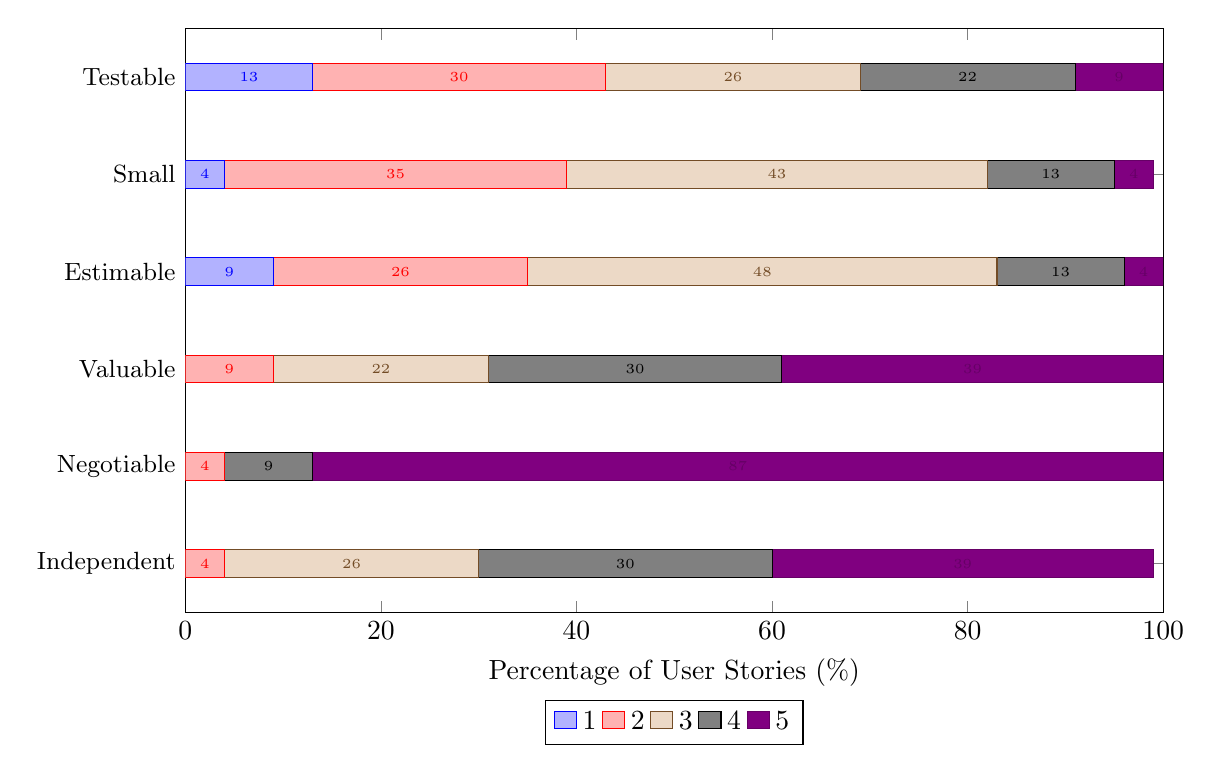
\begin{tikzpicture}
\begin{axis}[
    xbar stacked,
    width=14cm,
    height=9cm,
    xmin=0, xmax=100,
    xtick={0,20,40,60,80,100},
    xlabel={Percentage of User Stories (\%)},
    ytick=data,
    symbolic y coords={
        Independent,
        Negotiable,
        Valuable,
        Estimable,
        Small,
        Testable
    },
    yticklabel style={font=\small},
    legend style={
        at={(0.5,-0.15)},
        anchor=north,
        legend columns=5
    },
    nodes near coords,
    every node near coord/.append style={font=\tiny}
]

% Score 1
\addplot coordinates {(0,Independent) (0,Negotiable) (0,Valuable) (9,Estimable) (4,Small) (13,Testable)};
\addlegendentry{1}

% Score 2
\addplot coordinates {(4,Independent) (4,Negotiable) (9,Valuable) (26,Estimable) (35,Small) (30,Testable)};
\addlegendentry{2}

% Score 3
\addplot coordinates {(26,Independent) (0,Negotiable) (22,Valuable) (48,Estimable) (43,Small) (26,Testable)};
\addlegendentry{3}

% Score 4
\addplot coordinates {(30,Independent) (9,Negotiable) (30,Valuable) (13,Estimable) (13,Small) (22,Testable)};
\addlegendentry{4}

% Score 5
\addplot coordinates {(39,Independent) (87,Negotiable) (39,Valuable) (4,Estimable) (4,Small) (9,Testable)};
\addlegendentry{5}

\end{axis}
\end{tikzpicture}
\caption{Distribution of INVEST scores (Likert 1--5) across evaluated user stories}
\end{figure}


% TODO agregar imagen

\section{Aqusa}

La tabla de los defectos encontrados por Aqusa sobre las historias generadas por clickup

\begin{table}[h!]
\centering
\begin{tabular}{|c|c|p{8cm}|}
\hline
\textbf{Referencia HU} & \textbf{Defecto} & \textbf{Mensaje} \\
\hline
H7 & atomic.conjunctions & As an administrative staff member, I want to modify \textbf{or} cancel existing appointments, so that changes can be managed as needed. \\
\hline
H8 & atomic.conjunctions & As a patient, I want to receive notifications when my appointment is modified \textbf{or} canceled, so that I am always informed about my schedule. \\
\hline
H13 & atomic.conjunctions & As an administrator, I want to define \textbf{and} modify attention hours and activate \textbf{or} deactivate professionals for scheduling, so that doctor availability is accurately reflected. \\
\hline
H19 & atomic.conjunctions & As a pharmacist, I want to be notified when stock is low \textbf{or} items are about to expire, so that I can take timely action. \\
\hline
\end{tabular}
\caption{Defectos de Aqusa en historias de usuario ClickUp}
\end{table}

El único defecto encontrado es el de atomic.conjunction, en 4 de las 23 historias.

\[
\% atomic.conjunction_{ClickUp} = \frac{\# atomic.conjunction} {\# Historias} * 100 = 4 / 23 * 100 = 17.39\%  
\]


\label{sec:resultados-comparacion}

% \subsection{Diseño experimental}
% \subsubsection{Escenarios / casos de prueba}

% \subsection{Procedimiento de medición}
% \subsubsection{Cálculo de métricas automáticas}

% \subsection{Resultados por métrica}

% \subsection{Comparación entre enfoques}
% \subsubsection{Criterio de comparación}

% \subsubsection{Discusión}
